\chapter{三角函數\\簡單定義及演算}
\chapterauthor{黃裕盛}

\setcounter{section}{-1}
\section{引導}
我知道你們看到標題會覺得很@@,三角函數怎麼可能會簡單? \\
希望在這堂課之後,可以克服對他的恐懼 :) (希望是不要加深啦)

\section{觀念}
\subsection{相似}
\subsubsection{定義}
兩個三角形的對應角相等,而對應邊成比例。

\subsubsection{判別種類}
\begin{enumerate}
\item AA相似
\item SAS相似
\item SSS相似
\end{enumerate}

\subsection{畢氏定理}
\subsubsection{定義}
當一個三角形為直角三角形時,其兩股平方和等於斜邊長。 \\
怎麼說呢?如下圖: \\

\definecolor{wrwrwr}{rgb}{0.3803921568627451,0.3803921568627451,0.3803921568627451}
\definecolor{rvwvcq}{rgb}{0.08235294117647059,0.396078431372549,0.7529411764705882}
\newpage
\begin{figure}[H]
\centering
\begin{tikzpicture}[line cap=round,line join=round,>=triangle 45,x=1.5cm,y=1.5cm]
%\clip(-2.505849312497348,-1.2756636626591513) rectangle (6.856860587833347,3.6499707160434913);
\fill[line width=2pt,color=rvwvcq,fill=rvwvcq,fill opacity=0.10000000149011612] (0,3) -- (3,0) -- (0,0) -- cycle;
\draw[line width=2pt,fill=black,fill opacity=0.10000000149011612] (0.1698999741866448,0) -- (0.16989997418664482,0.1698999741866448) -- (0,0.1698999741866448) -- (0,0) -- cycle; 
\draw [line width=2pt,color=rvwvcq] (0,3)-- (3,0);
\draw [line width=2pt,color=rvwvcq] (3,0)-- (0,0);
\draw [line width=2pt,color=rvwvcq] (0,0)-- (0,3);
\begin{scriptsize}
\draw [fill=rvwvcq] (0,3) circle (2.5pt);
\draw[color=rvwvcq] (0.06509155833768435,3.1734256013559996) node {$A$};
\draw [fill=rvwvcq] (3,0) circle (2.5pt);
\draw[color=rvwvcq] (3.060517993516196,0.16999000458609542) node {$B$};
\draw [fill=wrwrwr] (0,0) circle (2.5pt);
\draw[color=wrwrwr] (0.06509155833768435,0.16999000458609542) node {$C$};
\draw[color=rvwvcq] (1.4346581904647575,1.507519990347626) node {$c$};
\draw[color=rvwvcq] (1.5307681295613944,0.2260541357258003) node {$a$};
\draw[color=rvwvcq] (0.15319233584293468,1.5956207678528767) node {$b$};
\draw[color=black] (0.5376320922294816,0.36220988277936933) node {$\alpha = 90\textrm{\degre}$};
\end{scriptsize}
\end{tikzpicture}
\caption{直角三角形} \vskip 10 pt
\label{fig:right-tri}
\end{figure}

\noindent
在$\rm \bigtriangleup ABC$內$a^2 + b^2 = c^2$,這就是畢氏定理喔。\\
當今證明畢氏定理的方法有太多種了,我還是講解最簡單的那一種吧。 \\
\begin{proof}
\end{proof}
\newpage

\section{定義}
\subsection{前提}
兩直角三角形若其中一銳角相等,則兩邊比值相同,而無關大小及位置(By AA相
似),如下圖: \\
$\because \angle C = \angle D = 90^{\circ}; \angle B = \angle E \therefore \overline{AC} : \overline{FD} = \overline{CB} : \overline{DE}$
\begin{figure}[H]
\centering
\begin{tikzpicture}[line cap=round,line join=round,>=triangle 45,x=1cm,y=1cm]
%\clip(-8.386803745862085,-2.0982104574476206) rectangle (11.193489106455077,8.202799041419008);
\fill[line width=2pt,color=rvwvcq,fill=rvwvcq,fill opacity=0.10000000149011612] (-3,3) -- (-1,0) -- (-3,0) -- cycle;
\fill[line width=2pt,color=rvwvcq,fill=rvwvcq,fill opacity=0.10000000149011612] (1,0) -- (5,0) -- (1,6) -- cycle;
\draw[line width=2pt,fill=black,fill opacity=0.10000000149011612] (-2.644687138062653,0) -- (-2.644687138062653,0.3553128619373469) -- (-3,0.3553128619373469) -- (-3,0) -- cycle; 
\draw[line width=2pt,fill=black,fill opacity=0.10000000149011612] (1.355312861937347,0) -- (1.355312861937347,0.3553128619373469) -- (1,0.3553128619373469) -- (1,0) -- cycle; 
\draw [line width=2pt,color=rvwvcq] (-3,3)-- (-1,0);
\draw [line width=2pt,color=rvwvcq] (-1,0)-- (-3,0);
\draw [line width=2pt,color=rvwvcq] (-3,0)-- (-3,3);
\draw [line width=2pt,color=rvwvcq] (1,0)-- (5,0);
\draw [line width=2pt,color=rvwvcq] (5,0)-- (1,6);
\draw [line width=2pt,color=rvwvcq] (1,6)-- (1,0);
\begin{scriptsize}
\draw [fill=rvwvcq] (-3,3) circle (2.5pt);
\draw[color=rvwvcq] (-2.859432795250738,3.3537872529281314) node {$A$};
\draw [fill=rvwvcq] (-1,0) circle (2.5pt);
\draw[color=rvwvcq] (-0.8662293312424045,0.355607252444999) node {$B$};
\draw [fill=rvwvcq] (-3,0) circle (2.5pt);
\draw[color=rvwvcq] (-3.479168326076859,0.33885764350375247) node {$C$};
\draw[color=rvwvcq] (-2.1726988286596316,1.544829487273504) node {$c$};
\draw[color=rvwvcq] (-1.9382043034821808,0.4728545150337249) node {$a$};
\draw[color=rvwvcq] (-2.6751870968970266,1.6955759677447229) node {$b$};
\draw [fill=rvwvcq] (1,0) circle (2.5pt);
\draw[color=rvwvcq] (0.5574874287635483,0.30535842562125937) node {$D$};
\draw [fill=rvwvcq] (5,0) circle (2.5pt);
\draw[color=rvwvcq] (5.130130669723844,0.355607252444999) node {$E$};
\draw [fill=rvwvcq] (1,6) circle (2.5pt);
\draw[color=rvwvcq] (1.1269741327659293,6.351967253411264) node {$F$};
\draw[color=rvwvcq] (3.0531791610092776,-0.0631329710861647) node {$f$};
\draw[color=rvwvcq] (3.2876736861867286,3.3537872529281314) node {$d$};
\draw[color=rvwvcq] (0.7919819539409994,3.2030407724569123) node {$e$};
\draw[color=black] (-2.0387019571296596,0.3221080345625059) node {$\alpha = 90\textrm{\degre}$};
\draw[color=black] (1.8807065351220222,0.3221080345625059) node {$\beta = 90\textrm{\degre}$};
\end{scriptsize}
\end{tikzpicture}
\caption{AA相似} \vskip 10pt
\label{fig:AA-tri}
\end{figure}

\subsection{定義}
\noindent
如下圖:$\overline{AC}$稱為$\angle A$的鄰邊,$\overline{BC}$稱為$\angle A$的對邊,$\overline{AB}$稱為斜邊。

\begin{figure}[H]
\centering
\begin{tikzpicture}[line cap=round,line join=round,>=triangle 45,x=1.5cm,y=1.5cm]
%\clip(-2.505849312497348,-1.2756636626591513) rectangle (6.856860587833347,3.6499707160434913);
\fill[line width=2pt,color=rvwvcq,fill=rvwvcq,fill opacity=0.10000000149011612] (0,3) -- (3,0) -- (0,0) -- cycle;
\draw[line width=2pt,fill=black,fill opacity=0.10000000149011612] (0.1698999741866448,0) -- (0.16989997418664482,0.1698999741866448) -- (0,0.1698999741866448) -- (0,0) -- cycle; 
\draw [line width=2pt,color=rvwvcq] (0,3)-- (3,0);
\draw [line width=2pt,color=rvwvcq] (3,0)-- (0,0);
\draw [line width=2pt,color=rvwvcq] (0,0)-- (0,3);
\begin{scriptsize}
\draw [fill=rvwvcq] (0,3) circle (2.5pt);
\draw[color=rvwvcq] (0.06509155833768435,3.1734256013559996) node {$A$};
\draw [fill=rvwvcq] (3,0) circle (2.5pt);
\draw[color=rvwvcq] (3.060517993516196,0.16999000458609542) node {$B$};
\draw [fill=wrwrwr] (0,0) circle (2.5pt);
\draw[color=wrwrwr] (0.06509155833768435,0.16999000458609542) node {$C$};
\draw[color=rvwvcq] (1.4346581904647575,1.507519990347626) node {$c$};
\draw[color=rvwvcq] (1.5307681295613944,0.2260541357258003) node {$a$};
\draw[color=rvwvcq] (0.15319233584293468,1.5956207678528767) node {$b$};
\draw[color=black] (0.5376320922294816,0.36220988277936933) node {$\alpha = 90\textrm{\degre}$};
\end{scriptsize}
\end{tikzpicture}
\caption{直角三角形} \vskip 10 pt
\label{fig:right-tri}
\end{figure}

\begin{figure}[H]
\centering
\graphicspath{{math/}}
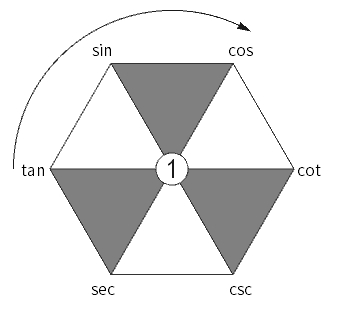
\includegraphics[width=5cm, center]{hex-tri.png}
\caption{神秘的三角函數六邊形} \vskip 10 pt
\label{fig:hex-tri}
\end{figure}

\begin{align*}
\sin A &= \frac{a}{c} \mbox{(稱作正弦值)} \\
\cos A &= \frac{b}{c} \mbox{(稱作餘弦值)} \\
\tan A &= \frac{a}{b} \mbox{(稱作正切值)} \\
\cot A &= \frac{b}{a} \mbox{(稱作餘切值)} \\
\sec A &= \frac{c}{b} \mbox{(稱作正割值)} \\
\csc A &= \frac{c}{a} \mbox{(稱作餘割值)} \\
\end{align*}
※這些名字可以不用記沒關係,然後建議背最上方三個然後倒數變成下面三個。

\subsection{三角函數間的關係}
\subsubsection{平方關係}
\begin{enumerate}
\item ${\sin}^2 + {\cos}^2 = 1$
\item $1 + {\tan}^2 = {\sec}^2$
\end{enumerate}
\subsubsection{相除關係}
\begin{enumerate}
\item $\tan \theta = \frac{\sin \theta}{\cos \theta}$ (尷尬只有這一個)
\end{enumerate}
\subsubsection{倒數關係}
\begin{enumerate}
\item $\sin \theta \cdot \csc \theta = 1$
\item $\cos \theta \cdot \sec \theta = 1$
\item $\tan \theta \cdot \cot \theta = 1$
\end{enumerate}
\subsubsection{餘角關係($90^\circ - \theta$)}
\begin{enumerate}
\item $\sin (90^\circ-\theta) = \cos \theta$;$\cos (90^\circ-\theta) = \sin \theta$
\item $\tan (90^\circ-\theta) = \cot \theta$;$\cot (90^\circ-\theta) = \tan \theta$
\item $\sec (90^\circ-\theta) = \csc \theta$;$\csc (90^\circ-\theta) = \sec \theta$
\end{enumerate}
※證明由圖 \ref{fig:hex-tri}就可以看出喔! \vskip 20 pt

\noindent
\fbox{小練習} \vskip 10 pt
\noindent
$\bigtriangleup ABC$的$\angle A$為銳角,$\angle C=90^\circ$,$\overline{AC}=10$;$\overline{AB}=26$,求$\angle A$的六個三角函數值。
\vspace{5cm}

\noindent
\fbox{小笑話} \vskip 10 pt
\noindent
sin對cos說:買這麼多衣服想玩甚麼?\\
cos說:我想玩cosplay \\


\noindent
\fbox{腦筋急轉彎} \vskip 10 pt
\noindent
$\frac{\sin x}{n} =$ ? \\
\rightline{Ans:6}

\section{講師介紹}
\begin{itemize}
\item 姓名:黃裕盛
\item 性別:男
\item 特色:大電神,非常認真、心算能力頂尖,可在2秒內算出四位數乘四位數、每天固定打一場LOL,但真的就只有打一場、對化學有興趣,跟熊熊借了熊熊很少在看的化學經典教材小銀、喜歡拿橡皮筋彈穿短褲的熊熊,並以此為樂。
\item 名言:這題講義出現過啊,我就直接寫答案了(編按:此為數學段考)。
\end{itemize}